\chapter{Status of Ceramic Breeder Modeling and Analysis}\label{sec:modeling-state}
A common problem plaguing those who study packed beds is the multi-scale of physics dictating the behavior of the packed bed. In the realm of engineering continuum mechanics, packed beds cannot be adequetly described as a solid or liquid (or obviously gas) alone. Under compression, a packed bed responds like a solid with non-linear elasticity and a plasticity that is history-dependent. The packed bed can obviously not support any tensile pressure and will often behave like a liquid as it may fill in voids under just the force of gravity. Experiments on packed beds provide effective material properties that are often specific to the material, packing fraction, moisture content, or level of polydispersity.

In packed beds of ceramics for tritium breeding, phenomenological models have been developed based on the controlled environment of laboratory experiments. The models provide reliable information on the initial states of breeder volumes in the fusion reactor environment and allow reasonable design predictions of the thermomechanics of the breeding blanket. Unfortunately, a certain measurable quantity in an experiment may arise due to vastly different pebble-scale physics. Furthermore, it is unavoidable that other morphological changes of the pebble bed may arise due to individual pebble cracking, inter-particle creep, or inter-particle sintering. Designers of solid breeder blankets must have predictive capabilities for the initiation of morphological changes in the packed bed as well as how those changes impact the thermophysics of the bed.

The solid breeder in many current designs feature sub-module units of packed beds. From the point of view of pebble bed thermomechanical properties, this has the advantage of producing units individually that can be tested and qualified to desired packing states (and therefore thermomechanics) during the design phase. 



The thermophysical and thermomechanical properties of pebble beds have been studied extensively [cite many of the experimental papers]. From experimental measurements, and the assumption that a pebble bed can be treated as a continuous media, researchers have developed phenomonological formulas relating properties of pebble bed to other, measurable, macroscopic properties [cite many of the modeling papers]. For instance, an effective thermal conductivity can be given for the packed bed given a certain gas and stress on the bed. These effective material properties are useful for the design and qualification of tritium breeding modules. But it must be understood that the material properties of a pebble bed are a function of their history and will evolve in time as the morphological features of the pebble bed likewise evolve in time. Therefore there is a need to predict the morphological changes to the pebble bed and the subsequent impact on the bed's thermophysical properties so that solid breeder designers may have reliable temperature control of the pebble bed over the duration of the use of the breeder in the reactor. 

^^ above is copied from old sections but seem more appropriate here
%~~~~~~~~~~~~~~~~~~~~~~~~~~~~~~~~~~~~~~~~~~~~~~~~~~~~~~~~~~~~~
Ceramic breeders, by their nature, are brittle and prone to cracking under external mechanical loadings. These breeders, in the form of packed beds of pebbles, are loaded into a box-like structure for tritium fuel production in a fusion reactor. When subjected to nuclear heating in a reactor, a strong mechanical loading arises from the differential thermal expansion between breeder pebbles and their containing structure. Research efforts have therefore been aimed at developing a thorough understanding and characterization of the ceramic breeder pebble bed thermomechanics. Such an understanding is essential to providing confidence in the performance and lifetime of a ceramic breeder blanket design. In particular, a significant effort of the pebble bed thermomechanics study is on the development of modeling simulation tools. 

Reimann, et al. have conducted an extensive experimental study of the stress-strain relations of the ceramic breeder pebble beds using an oedometric test apparatus \cite{Piazza2002811,Reimann:2002kl,Reimann:2003qc,Reimann:2002mi,Reimann:2001il}. The most significant macroscopic experimental phenomena witnessed in the pebble bed are an irreversible plastic strain when the load is removed, a non-linear elasticity, a pressure-dependent plasticity, and a volumetric creep.  A particularly noticeable feature, clearly demonstrated in Fig.~\ref{fig:mti}, is the reduced amount of irreversible strain when subjected to additional loading cycles after the first unloading. This may suggest the existence of a semi-equilibrium packing state in the pebble bed which can be reached after applying a pre-load to account for the large strain in the first cycle of a pebble bed. This semi-equilibrium packing state is a feature which may be advantageous for use in a fusion reactor. 

To study the temperature effect in Reimann's studies, the bed is freely heated to the desired working temperature before the pressure load is applied. Under the same loading condition, the bed behaves much softer at higher temperatures. The bed stiffens as the pressure increases. An illustration of this phenomenon is presented in Fig.~\ref{fig:UCT} for a lithium orthosilicate pebble bed between $50-850^\circ$C. At higher temperatures (such as $> 650^\circ$C), a creep-like behavior becomes apparent. The creep behavior allows the pebble bed to relax and sustain higher stresses, however one needs to avoid sintering. The data was used to correlate creep rate as a function of temperature, stress, and time for both lithium orthosilicate, lithium metatitanate, and beryllium pebble beds \cite{Buhler:2002qf,Reimann:2001il,Reimann:2005qa}.


\begin{figure}[t!]
\begin{center}
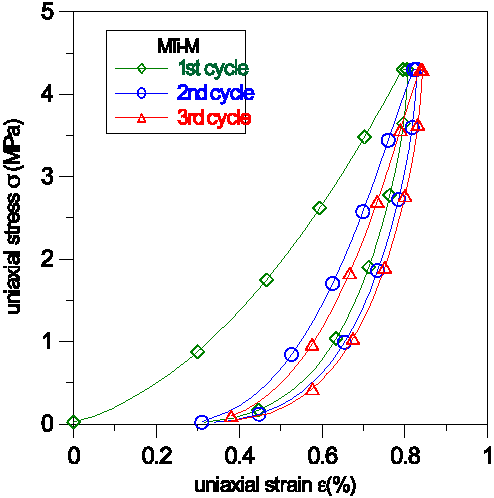
\includegraphics[width=0.4\textwidth]{chapters/figures/Fig-1}
\caption{Example of uniaxial compression testing results for lithium metatitanate pebble bed \cite{vanderlaan2011}.}
\label{fig:mti}
\end{center}
\end{figure}

\begin{figure}[t!]
\begin{center}
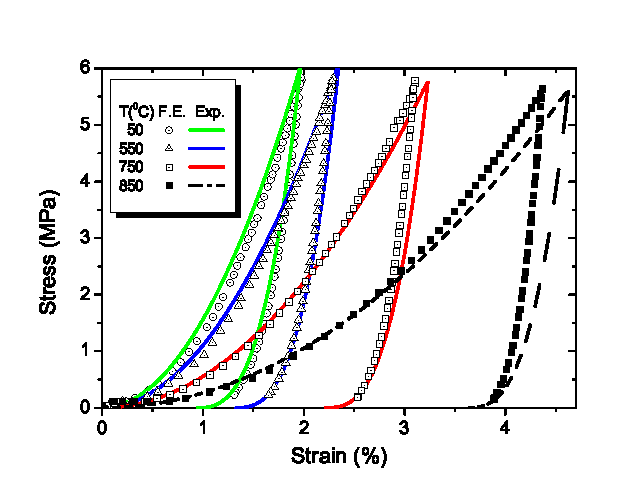
\includegraphics[width=0.5\textwidth]{chapters/figures/Fig-2}
\caption{Example of uniaxial compression testing results compared with predictions from material constitutive equations for lithium orthosilicate pebble beds at different temperatures \cite{Gan:2008kx}.}
\label{fig:UCT}
\end{center}
\end{figure}

Phenomenological models, derived from the volumes of collected data, have been proposed to describe the aforementioned mechanical behavior of the pebble beds with a conventional continuum-based approach. The continuum approach allows treatment of the pebble beds with standard finite element modeling (FEM). To employ FEM, mathematical models written in terms of average quantities and containing effective parameters are used. These models deduce a set of constitutive equations to be implemented in the framework of a finite element code.  There are two major variants of phenomenological modeling approaches developed among institutions, including: (1) A non-linear elastic model and a modified Drucker-Prager-Cap theory for plastic strain \cite{Gan2007189,fokkens2003}; and (2) A hyperporous non-linear elastic model and a Gurson model for plastic model \cite{DellOrco:2007hc,DellOrco:2010zr,DiMaio20081287}. The readers are referred to the additional efforts used in a third method\cite{fokkens2003} which employed two different elasticity laws for the loading and unloading branches but will not be discussed here. Alongside the development of the modeling techniques, several large scale pebble bed thermomechanics experiments were conducted in parallel. These experiments were intended to reveal the underlined thermo-mechanical characteristics of ceramic breeder pebble beds, and provide data for benchmarking the developed models.   The validation statuses as well as the features of the models are briefly described in the following section. 

Another modeling strategy is to model the pebble bed as a system of distinct interacting bodies that are subject to forces and resulting motions. This modeling approach called discrete element modeling (DEM) considers the mechanical interaction between pebbles and numerically solves the associated equations of motion \cite{An20072233,An20071393,Gan:2010uq,Gan20101782}. The DEM approach has recently received increased attention and the progress will be summarized to follow.

The review of the current status of development on the ceramic breeder pebble bed thermomechanics is organized as follows. In Section 2, current continuum modeling approaches and constitutive models for mechanical and thermal interactions are presented. In Section 3, a review of recent advancements on DEM is presented. A brief discussion on recently-initiated benchmarking efforts, in-pile experimental results, and other experimental observations relevant to pebble bed thermomechanics are given in Section 4. A proposed framework and a few conclusions on the outlook are drawn in Section 5. 


%%%%%%%%%%%%%%%%%%%%%%%%%%%%%%%%%%%%%%%%%%%%%%%%%%%%%%%%%%%%%%%%%%%%%%%%%%%%%%%%%%%%%%%%%%%%%%%%%%%%%%%%%%%%%%%%%%%%%%%%%%%%%%%%%%%%%%%%%%%%%%%%%%%%%%%%%%%%%%%%%%%%%%%%%%%%%%%%%%%%%%%%%%%%%%%%%%%%%%%%%%%%%%%%%%%%%%%%%%%%%%%%%%%%%%%%%%%%%%%%%%%%%%%


\section{Status of Continuum Modeling Approaches}
\subsection{Mechanical constitutive equations}
Continuum models focus on predicting global behavior, including volumetric strain and stress and the impact on the effective thermal conductivity, etc. Two institutions in Europe have spearheaded modeling efforts. One being Karlsruhe Institute of Technology, formerly FZK and referred to as such throughout this paper, and the other being ENEA-Brasimone with the Department of Nuclear Engineering at the University of Palermo, referred to as DIN throughout this paper. These two institutions have published a great deal of detail in regards to the specific details of their modeling techniques and the reader is referred to these publications for the fine points of the models \cite{DellOrco:2007hc,DellOrco:2010zr,DiMaio20101234,Gan2007189}. The discussion here calls attention to differences between models and attempts to serve as a reference basis for future modeling efforts.

The models from FZK and DIN share a common treatment of the mechanical interaction between the pebble beds with structural walls. In models from the two institutes, interfacial contact and friction forces are taken into account by application of the Coulomb friction law. This frictional contact law can be simply implemented in finite element code without considerable computation effort.

\subsubsection{FZK mechanical model}
In the FZK approach, the corresponding phenomenological constitutive models were developed based on the soil mechanics models implemented in the finite element code ABAQUS. This includes a non-linear elasticity model, which was originally developed for powder die compaction; a plastic strain model via a modified Drucker-Prager-Cap model, which was originally developed for soil mechanics; time-dependence via a consolidation creep law; and global thermal-mechanical coupling from material parameters.

The Drucker-Prager-Cap model captures the plasticity of the pebble beds and predicts the yielding and hardening behavior. A feature of the classic Druger-Prager-Cap model, as implemented in ABAQUS, is the ability to describe the plastic behavior of pebble beds under hydrostatic compression; a feature which is not present in classical metal plasticity models. However, researchers at FZK recognized that for materials with large creep strain amplitudes (e.g. beryllium pebble beds), hardening laws defined by default in ABAQUS were insufficient. Therefore, unique hardening laws were developed and implemented in place of the standard equations referenced in ABAQUS. An advantage gained from the redefined hardening laws is their capture of the creep behavior witnessed in pebble beds at high temperatures. The disadvantage of the Drucker-Prager-Cap model is the computational resources necessary for convergence of solutions. This has so far limited the FZK model to spatially two-dimensional simulations.

The main distinguishing feature unique to the continuum model developed in FZK is in their treatment of the material parameters that feed into the models described above. In particular, the hardening law in the model is manipulated to accommodate direct fitting to the oedometric tests. Unlike other continuum models, which require a trial-and-error method of optimizing numeric elasto-plastic parameters, the FZK model can be directly and clearly linked to experimental data. In this way, the model may be most adept at predicting behavior of a pebble beds where stress and temperature fields are very different from the controlled experiments which produced the constitutive relationships \cite{Gan2007189,Gan:2009vn,Gan:2010lh,Gan:2010kc}.

\subsubsection{DIN mechanical model}
The mechanical model established in the DIN model similarly assumes a non-linear elasticity model and a plasticity model. The non-linear elastic model assumes that during the reversible straining of a pebble bed, its effective logarithmic bulk modulus depends on the equivalent pressure according to a hypothesized power law. From this assumption as the foundation, DIN proceeds through a semi-theoretical derivation to relate the bed deformation modulus to the equivalent pressure; and stress state to volumetric strain. Included in the derivation are a number of effective parameter values. Values of all material parameters are chosen on an iterative trial-and-error basis until the model agreed well with the non-linear, elastic curves seen in oedometric experiments.

Attempting to resolve large computing time required when using the Drucker-Prager-Cap model for plastic deformation, DIN instead used a Gurson model. The Gurson model was originally developed for the analysis of pressure-dependent plastic behavior of mildly voided materials. The Gurson model postulates that the pebble bed behavior can be modeled as a continuous matrix in which stochastically-distributed voids are contained. In the Gurson model, compaction-related plastic deformation of the bed can to be reproduced. For material parameters in the Gurson model, again an iterative procedure was used until the model reproduced the results of relevant experimental tests. Lastly, in the consideration of the effective hardening law in pebble beds, a fifth order polynomial function was hypothesized. It should be noted that in the model's current form, it is incapable of directly capturing the creep behavior of pebble beds. However, the model was designed such that a future creep law could readily be implemented \cite{DellOrco:2007hc,DellOrco:2010zr,DiMaio20101234}.

The main advantage of the approach taken by DIN in their model is apparent when considering computational demand. DIN is currently able to model three-dimensional experiments with modest computer time. The most apparent drawback is the ad-hoc procedure of determining effective parameters used in the model. Without a direct link to experimental data, the applicability of the chosen effective parameters at predicting behavior beyond the range of the experimental conditions is unknown.

\subsection{Mechanics and heat transfer coupling}
Maintaining the breeder temperature within its temperature window is crucial for predictable performance and lifetime of the breeder unit. Proper temperature analysis requires careful characterization of thermal properties of the pebble beds. 

The pebble-bed experiments demonstrated that the effective thermal conductivity depends on the volumetric compressive strain; changes in thermal conductivity occurred between compacted and un-compacted systems. These measured phenomena indicate that thermo-mechanical modeling must also consider full, non-linear coupling between thermal and mechanical analysis.

The thermal models of the two institutions are fundamentally similar. The form of thermal model used by FZK follows from the experimental work carried out by J. Reimann from FZK in which empirical equations have been reported where the temperature and volumetric inelastic strain-dependence is incorporated into the bulk thermal conductivity. The thermal conductivity for a lithiated ceramic pebble bed over a specified range of temperature is reported in Ref.~\cite{Gan2007189} as:
\begin{align}\label{eq:fzkK}
k \left(W/m \cdot K \right)& = 1.81+0.0012  \,T - 5 \times 10^{ - 7} \,T^2 + \nonumber\\
&+ \big(9.03-1.386\times10^{-3} \,T-7.6\times10^{-6}\, T^2 + \nonumber\\
&+ 2.1\times10^{-9} \,T^3\big)\epsilon
\end{align}
where $T$ and $\epsilon$ are the local temperature and strain, respectively. The formula for thermal conductivity owes its functional form to the widely used Schlunder, Zehner, and Bauer (SZB) model. The coefficients in Eq.~\eqref{eq:fzkK} are empirically derived from experiments. The FZK model has  linked its constitutive equations directly to experimental data. 

In the DIN thermal model, the effective thermal conductivity has a quasi-linear dependence on volumetric strain and temperature. DIN reports the equation for determining thermal conductivity in Ref.~\cite{DellOrco:2007hc}, it is:
\begin{align}\label{eq:dinK}
k\left(W/m \cdot K \right)&=\lambda_0\left(1+\gamma T+\delta \epsilon\right)
\end{align}
where T and $\epsilon$ are the local temperature and strain, respectively. The relationship of Eq.~\eqref{eq:dinK} introduces several effective parameters, $\lambda_0$, $\gamma$, and $\delta$, that are determined from iterative fits to experimental data. Values of these effective parameters have been determined thus far for beryllium and certain lithium orthosilicate pebble beds\cite{DiMaio20101234}. The thermal conductivity, being a function of both thermal and mechanical parameters endows the models with a full coupling between thermo-mechanical analyses. 

\subsubsection{Thermal interface model}
The thermal interaction at the interface between pebble bed and containment wall is represented in both models as an effective heat transfer conductance, with only slight variations between the two approaches. In the FZK model, the thermal interaction is simulated with an effective heat transfer coefficient. The heat transfer coefficient (HTC) incorporates the combined effects of radiation heat transfer, pebble-solid conduction, and solid-gas heat transfer. Furthermore, in the event of a gap formation at the interface between pebble bed and containing surface, a separate heat transfer coefficient is employed. The researchers at DIN noted that interface conductance is affected by parallel paths of heat flow: pebble-wall conduction at contact areas and gas-wall convection. DIN therefore posits that the macroscopic phenomena can be modeled as a pressure-dependent thermal gap at the interface. They therefore have a thermal interface conductance that is a function of temperature, pressure, and local volumetric strain. An iterative trial-and-error method was also used to determine the effective parameters in this term. 


%%%%%%%%%%%%%%%%%%%%%%%%%%%%%%%%%%%%%%%%%%%%%%%%%%%%%%%%%%%%%%%%%%%%%%%%%%%%%%%%%%%%%%%%%%%%%%%%%%%%%%%%%%%%%%%%%%%%%%%%%%%%%%%%%%%%%%%%%%%%%%%%%%%%%%%%%%%%%%%%%%%%%%%%%%%%%%%%%%%%%%%%%%%%%%%%%%%%%%%%%%%%%%%%%%%%%%%%%%%%%%%%%%%%%%%%%%%%%%%%%%%%%%%



\section{Discrete Element Method}
Discrete Element Method (DEM) introduced by~\cite{Cundall1979} has been shown to be a promising tool to study the behavior of granular systems through the interaction between the individual particles. DEM has been used successfully to study the micromechanical aspects of pebble bed thermo-mechanics in the past~\cite{An20072233,Gan:2010uq}. Furthermore, DEM can be used to establish a relation between the microscopic interactions and the macroscopic response of the granular assemblies. Reference \cite{An20072233} studied the pebble assemblies in rectangular and cylindrical containers bounded by a elastic walls. The effect of packing factor, geometry of the assembly on the overall stress-strain response under uni-axial compression tests (UCT) has been thoroughly investigated. \cite{Gan:2010uq} have studied similar pebble assemblies in a cubic box with periodic boundary conditions. In both the above studies, a non-linear stress-strain response and a characteristic residual strain after unloading (analogous to plastic strain in continuum systems) has been observed akin to the experimental results~\cite{Reimann:2000tw}. It has been shown that the average coordination number, average normal contact force and the maximum normal contact force in the assembly has a unique functional relation (nonlinear, linear and linear, respectively) with the hydrostatic pressure or the applied pressure independent of the packing factor~\cite{Gan:2010uq,An20071393}. These functional relations may be used as master curves for the micro-macro correspondence in the pebble bed thermo-mechanics studies. A first attempt to include the creep mechanism in DEM has been made by~\cite{An20071393} showing the experimentally observed phenomenon such as the reduction of creep strain rate over time under constant load, albeit qualitatively. Further advances in the thermo-mechanics of pebble beds using DEM are under progress at KIT and UCLA in collaboration with experiments.

Recently, the effect of the pebble size distribution on the overall thermo-mechanical behavior of the pebble assembly is studied by~\cite{Annabattula2011} considering the pebble size distribution of ceramic breeder pebbles (Orthosilicate (OSi) pebbles) with a diameter range of $0.25\ \mathrm{mm}$-$0.65\ \mathrm{mm}$. Figure~\ref{fig:pebble-assembly-potential-energy} shows a binary pebble assembly in a periodic box. The colors indicate stored elastic strain energy of the pebble (red: maximum and blue: zero). The assembly has a maximum pebble radius $\rmax=0.25$ mm with the pebble size ratio $\rstar=\rmin/\rmax=0.6$, relative volume fraction $\vstar=\vmax/V=0.7$ and a packing factor $\eta=0.643$. The average stress in a granular assembly can be deduced from the contact forces between individual grains.

Another aspect of interest in the study of mechanics of pebble beds is the crush behavior of individual pebbles and their impact on the over all pebble bed response. DEM is used to study the behavior of a crushable pebble assembly with the crush load data for OSi pebbles (for individual pebbles) measured at KIT for pebbles of diameter 0.5 mm. 

A probabilistic method for analyzing the crush events of individual pebbles and a procedure with the combination of DEM and experimental data to obtain crush load probability has been reported by~\cite{Gan:2010kc}. Figure~\ref{fig:cdf_pebbles} shows the cumulative distribution function as a function of the hydrostatic pressure placed on the bed. The probability analysis, derived from DEM calculations, provides quantitative report of pebble crushing as a function of a specific hydrostatic pressure. The results of this analysis exemplify the growing strength of DEM techniques for analyses connecting global pebble bed loads to individual pebbles.

However, it has been shown~\cite{Zhao2010,Zhao2011} that a criterion based on critical stored elastic energy is the most suitable criterion for describing the OSi pebble failure. Hence, the crush load data (provided by fusion materials laboratory at KIT) has been transformed into equivalent elastic strain energy showing a Weibull distribution~\cite{Zhao2010}. This critical energy (randomly generated distribution) is used as the criterion for failure of pebbles in the DEM simulations. First, the assembly is loaded up to 3\% strain in uniaxial compression and then unloaded to a stress-free state. The elastic modulus of the pebble is reduced (from initial value to a small value of 1 kPa) with increase in elastic strain energy of the pebble according to a phenomenological damage accumulation law~cite{Annabattula2011b}. The damage state is frozen at the end of loading step and hence there will be no further damage accumulation in the unloading step. 

Figure.~\ref{fig:stress-strain-effect} shows the results for two types of damage law each with three different realizations. Each realization corresponds to a different random distribution of critical energies assigned to the pebbles in the assembly. The results do not show appreciable sensitivity to random distribution of energies. In the case of gradual damage law, the reduction of the elastic modulus of the pebble starts when the stored elastic energy reaches 50\% of the critical energy for that pebble and the elastic modulus reaches exponentially to its minimum value when the stored elastic energy reaches the critical energy prescribed. In the case of sudden damage this reduction starts at a much later stage when the stored elastic energy reaches 95\% of the critical energy of the pebble. Clearly, the assembly with a sudden damage accumulation shows a higher maximum strength compared to the gradual damage. In the case of the gradual damage, the pebbles start to degrade much earlier (at small strain) than in the case of sudden damage. Hence the critical number of pebbles to fail for the onset of maximum strength is reached earlier (at small strain) in gradual damage. It turns out that a mere 0.2\% pebbles is the critical number for the onset of maximum strength (stress plateau) observed. 

The nature of damage evolution influences the maximum strength and strain at which the maximum strength is attained while the critical number of failed pebbles for this saturation is independent of the damage evolution law (also see~\cite{Zhao2010}). Also note that the high frequency oscillations during loading in the stress-plateau region represent the failure of new pebbles. The current analysis also shows a creep-like behavior of the stress-strain response and hence the stress-plateaus observed in the experiments~\cite{Reimann:2000tw} may indicate the presence of pebble crushing in addition to the thermal creep mechanism. Furthermore, the residual strain after unloading is large for the system with sudden damage than the system with gradual damage. It should be noted that the assembly with gradual damage has more number of damaged pebbles at the end of loading (at 3\% strain) making the assembly more compliant than in the case of sudden damage. 


%%%%%%%%%%%%%%%%%%%
\begin{figure}
\begin{center}
\begin{minipage}{0.45\textwidth}
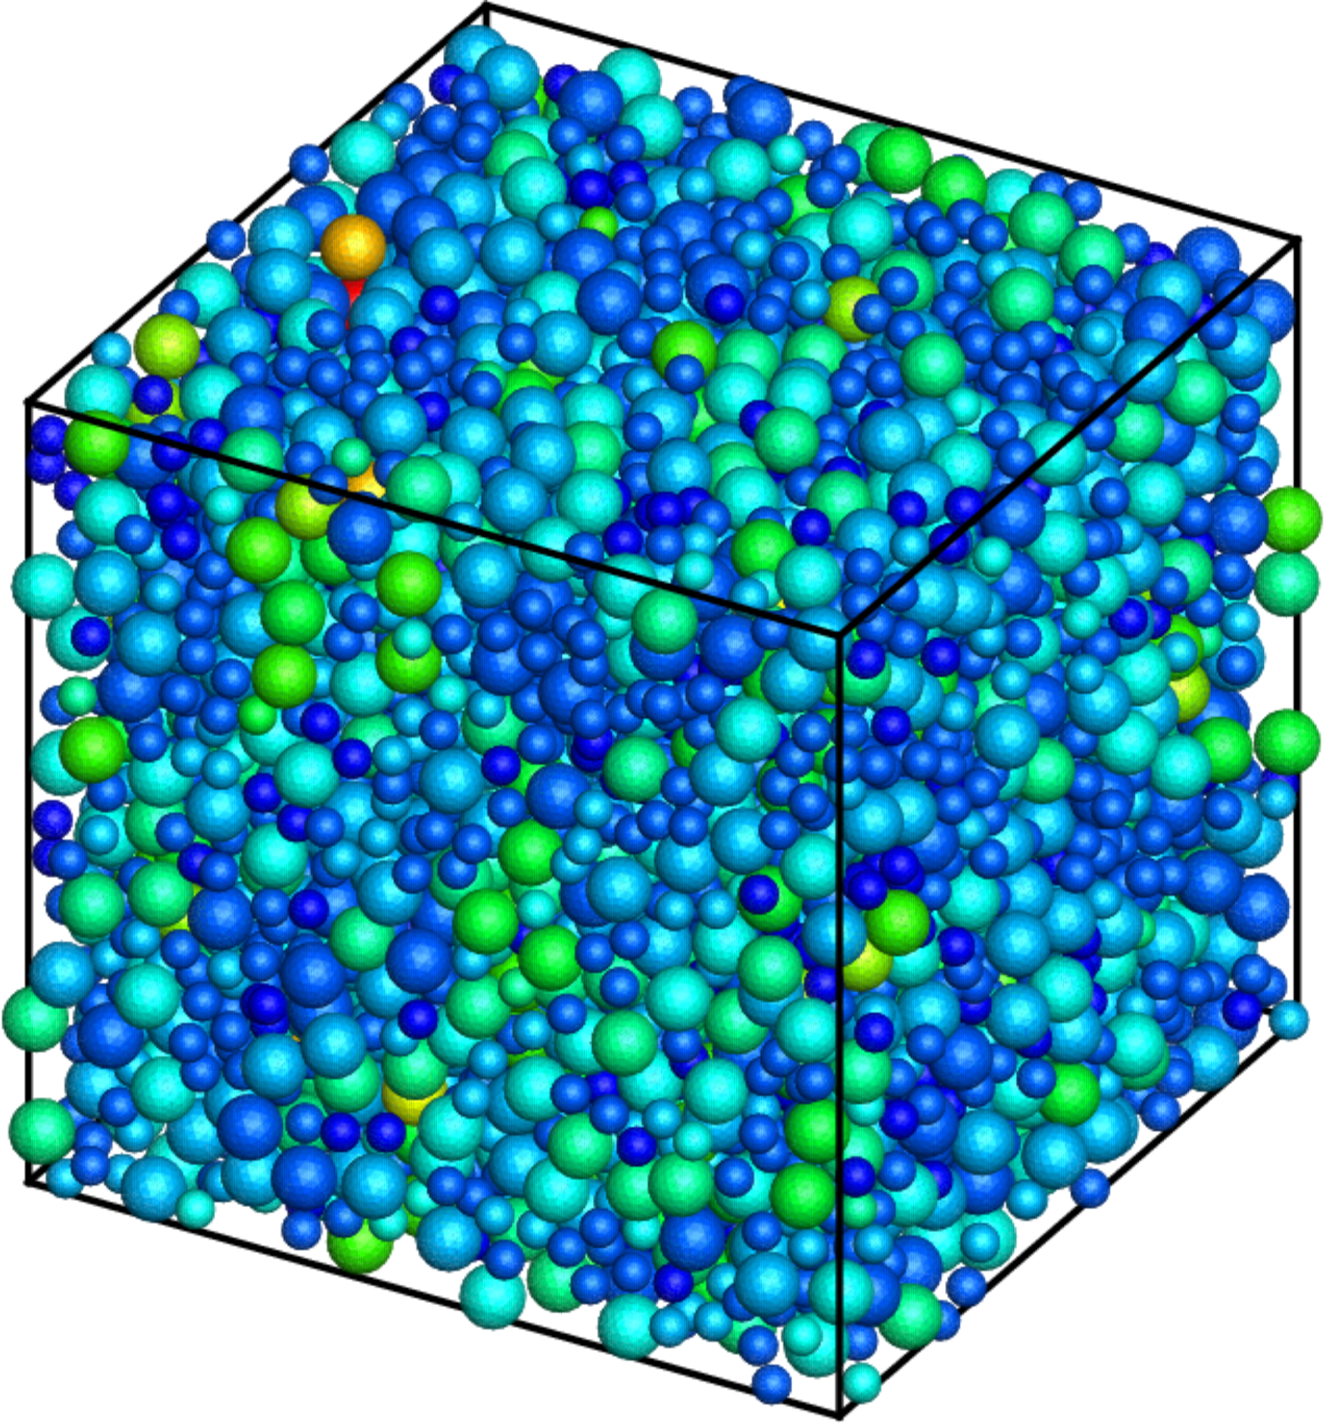
\includegraphics[width=6cm]{chapters/figures/Fig-3}
\begin{picture}(15,15)(340,-120)
\put(330,-80){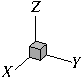
\includegraphics[scale=1]{chapters/figures/Fig-3b}}
\end{picture}
\end{minipage}
\end{center}
\caption{(color online) A binary pebble assembly with $\rstar = 0.6$ and $\vstar=0.7$ showing the stored elastic energy of the pebbles at $\epsilon_{33}=1.5\%$; pebbles of radius $r_s$ (small) and $r_g$ (large).}
\label{fig:pebble-assembly-potential-energy}
\end{figure}



\begin{figure}[!t]
  \begin{center}
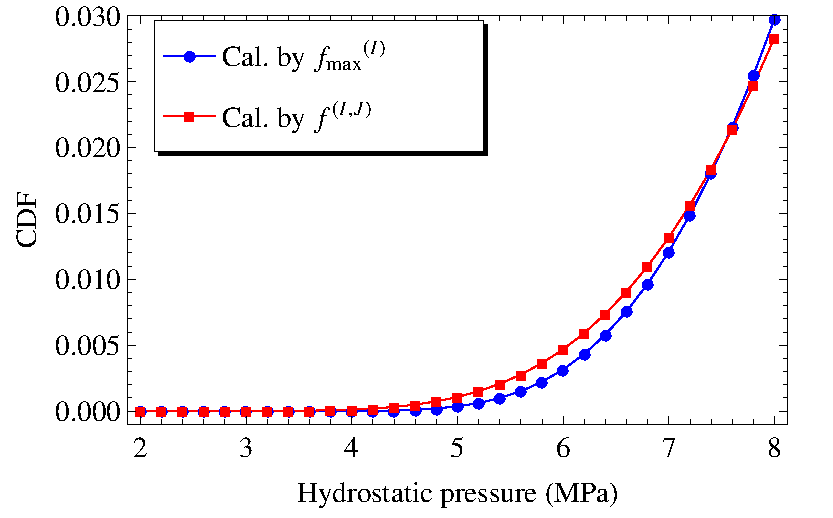
\includegraphics[width=0.5\textwidth]{chapters/figures/Fig-4}
\end{center}
 \caption{(color online) Cumulative distribution functions for crushing of individual pebbles inside the bed for as-fabricated pebbles, calculated by (1) maximum contact forces and (2) all inter-particle contact forces~\cite{Gan:2010kc}.}
 \label{fig:cdf_pebbles}
\end{figure}


\begin{figure}[t!]
\begin{center}
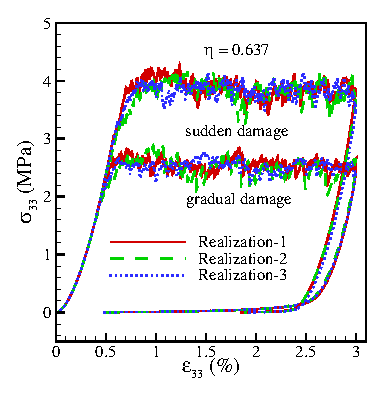
\includegraphics[width=0.4\textwidth]{chapters/figures/Fig-5}
\end{center}
\caption{(color online) Stress-Strain response of a granular assembly under uni-axial compression for two different damage evolution laws (gradual and sudden). Each damage evolution criterion is simulated with three different realizations of randomly prescribed critical failure energy for individual pebbles following Weibull distribution.}
\label{fig:stress-strain-effect}
\end{figure}



\section{Experimental Pebble Bed Thermomechanics Studies}
\subsection{Out-of-pile experiments}
The constitutive equations developed for finite element models were derived from the uniaxial compression experiments, which are not fully representative of fusion operating conditions. A more prototypical experiment should subject a pebble bed to isostatic loading. This could be generated by either an in-pile pebble bed experiment or by making use of differential thermal expansion between a pebble bed and its containing structure. The latter has been attempted with several out-of-pile experiments launched by the HE-FUS 3 facility at ENEA Brasimone. The experiments investigated the thermo-mechanical behavior of pebble beds within geometry much more representative of current breeder designs. These include the medium-scale mock-up exercises of HELICA (HE-FUS3 Lithium Cassette) and HEXCALIBER (HE-FUS3 Experimental Cassette of Lithium Beryllium Pebble Beds) \cite{dellorco:2006,DiMaio20081287}. For those experiments, the pebble layers are heated by electric heaters, and temperature and displacement were measured.

\subsubsection{FZK Benchmarking}
FZK has performed validation of their FEM code against the data collected from the HELICA experiment \cite{Gan:2008kx}. They have also reported the results of simulations of HEXCALIBER but have, as yet, not directly validated against the collected experimental data \cite{Gan:2009vn}.

In the HELICA experiment, the pebble beds experienced six thermal ramps, each applied for an hour, and then the pebble beds were actively cooled with a helium flow. After cooling, the pebble beds were subjected to the another thermal ramp and the process was repeated. DIN reports\cite{dellorco:2006} that the pebble bed temperatures exhibited cyclical behavior. FZK simulated two cycles of the HELICA test and an example of the calculated results and experimental data are shown in Fig.~\ref{fig:FZK_HELICAa} and Fig.~\ref{fig:FZK_HELICAb}. In Fig.~\ref{fig:FZK_HELICAa} we see temperature histories at a particular location (100 mm from the first wall) during a loading-unloading cycle. The simulation results follow the temperature increase during the thermal ramps up until the seventh hour, then again follow the experimental data as the test rig is cooled with the helium coolant. Even with the two-dimensional simplification of the model, there is excellent agreement between calculations and measurements. In Fig.~\ref{fig:FZK_HELICAb} the displacement calculated by FZK is also in strong agreement with the average of measured displacements for the entire duration of the heating-cooling cycle. Because of the overwhelming amount of computer time necessary for the FZK model to complete a fully three-dimensional and transient simulation, the FZK computations of HELICA and HEXCALIBER are carried out in two dimensions; the helium temperature is chosen at an average value of measured inlet and outlet temperatures.

From FZK's numeric simulation arise several important observations: (i) a three-dimensional analysis would provide more detail, spatial temperature variation of e.g. coolants would likely explain much of the deviation between temperature profiles predicted by the simulation and measured in the HELICA experiment; (ii) gap formations, with sizes on the order of a pebble diameter, were detected at the interface of the first wall in ceramic beds; (iii) the maximum hydrostatic pressures seen in the ceramic bed are anticipated to be above the fracturing limit of the lithium ceramic. The consequences of some of these observations, if true and real, are severe enough that they merit careful attention. Gap formation and pebble failure (crush or fracturing) are important topics that must be considered in validation with future experiments.

\subsubsection{DIN Benchmarking}
Because of the characteristics of the DIN model, full three-dimensional simulations were capable of being relatively easily performed. In the framework of benchmarking efforts, DIN has performed validation of their model against experimental results of HELICA, shown in Fig.~\ref{fig:DIN_HELICA} as well as HEXCALIBER, shown in Fig.~\ref{fig:DIN_HEX}.

The results of the DIN model show also strong agreement to the experimental results of HELICA as demonstrated in one example of temperature histories shown in Fig.~\ref{fig:DIN_HELICA}. In this profile, the same location as that modeled by FZK (100 mm from the first wall) is simulated by DIN. The FEM simulations from DIN (Fig.~\ref{fig:DIN_HELICA}) are reported over the six-hour heating portion of a single heating ramp cycle of HELICA. When comparing the results from DIN with those of FZK (in Fig.~\ref{fig:FZK_HELICAa} and Fig.~\ref{fig:FZK_HELICAb}) we see the DIN model has slightly better predictive capabilities for the temperature histories. This may be due attributed to the three-dimensional variations in coolant temperature being captured by the DIN model. 


\begin{figure}[t!]
\centering
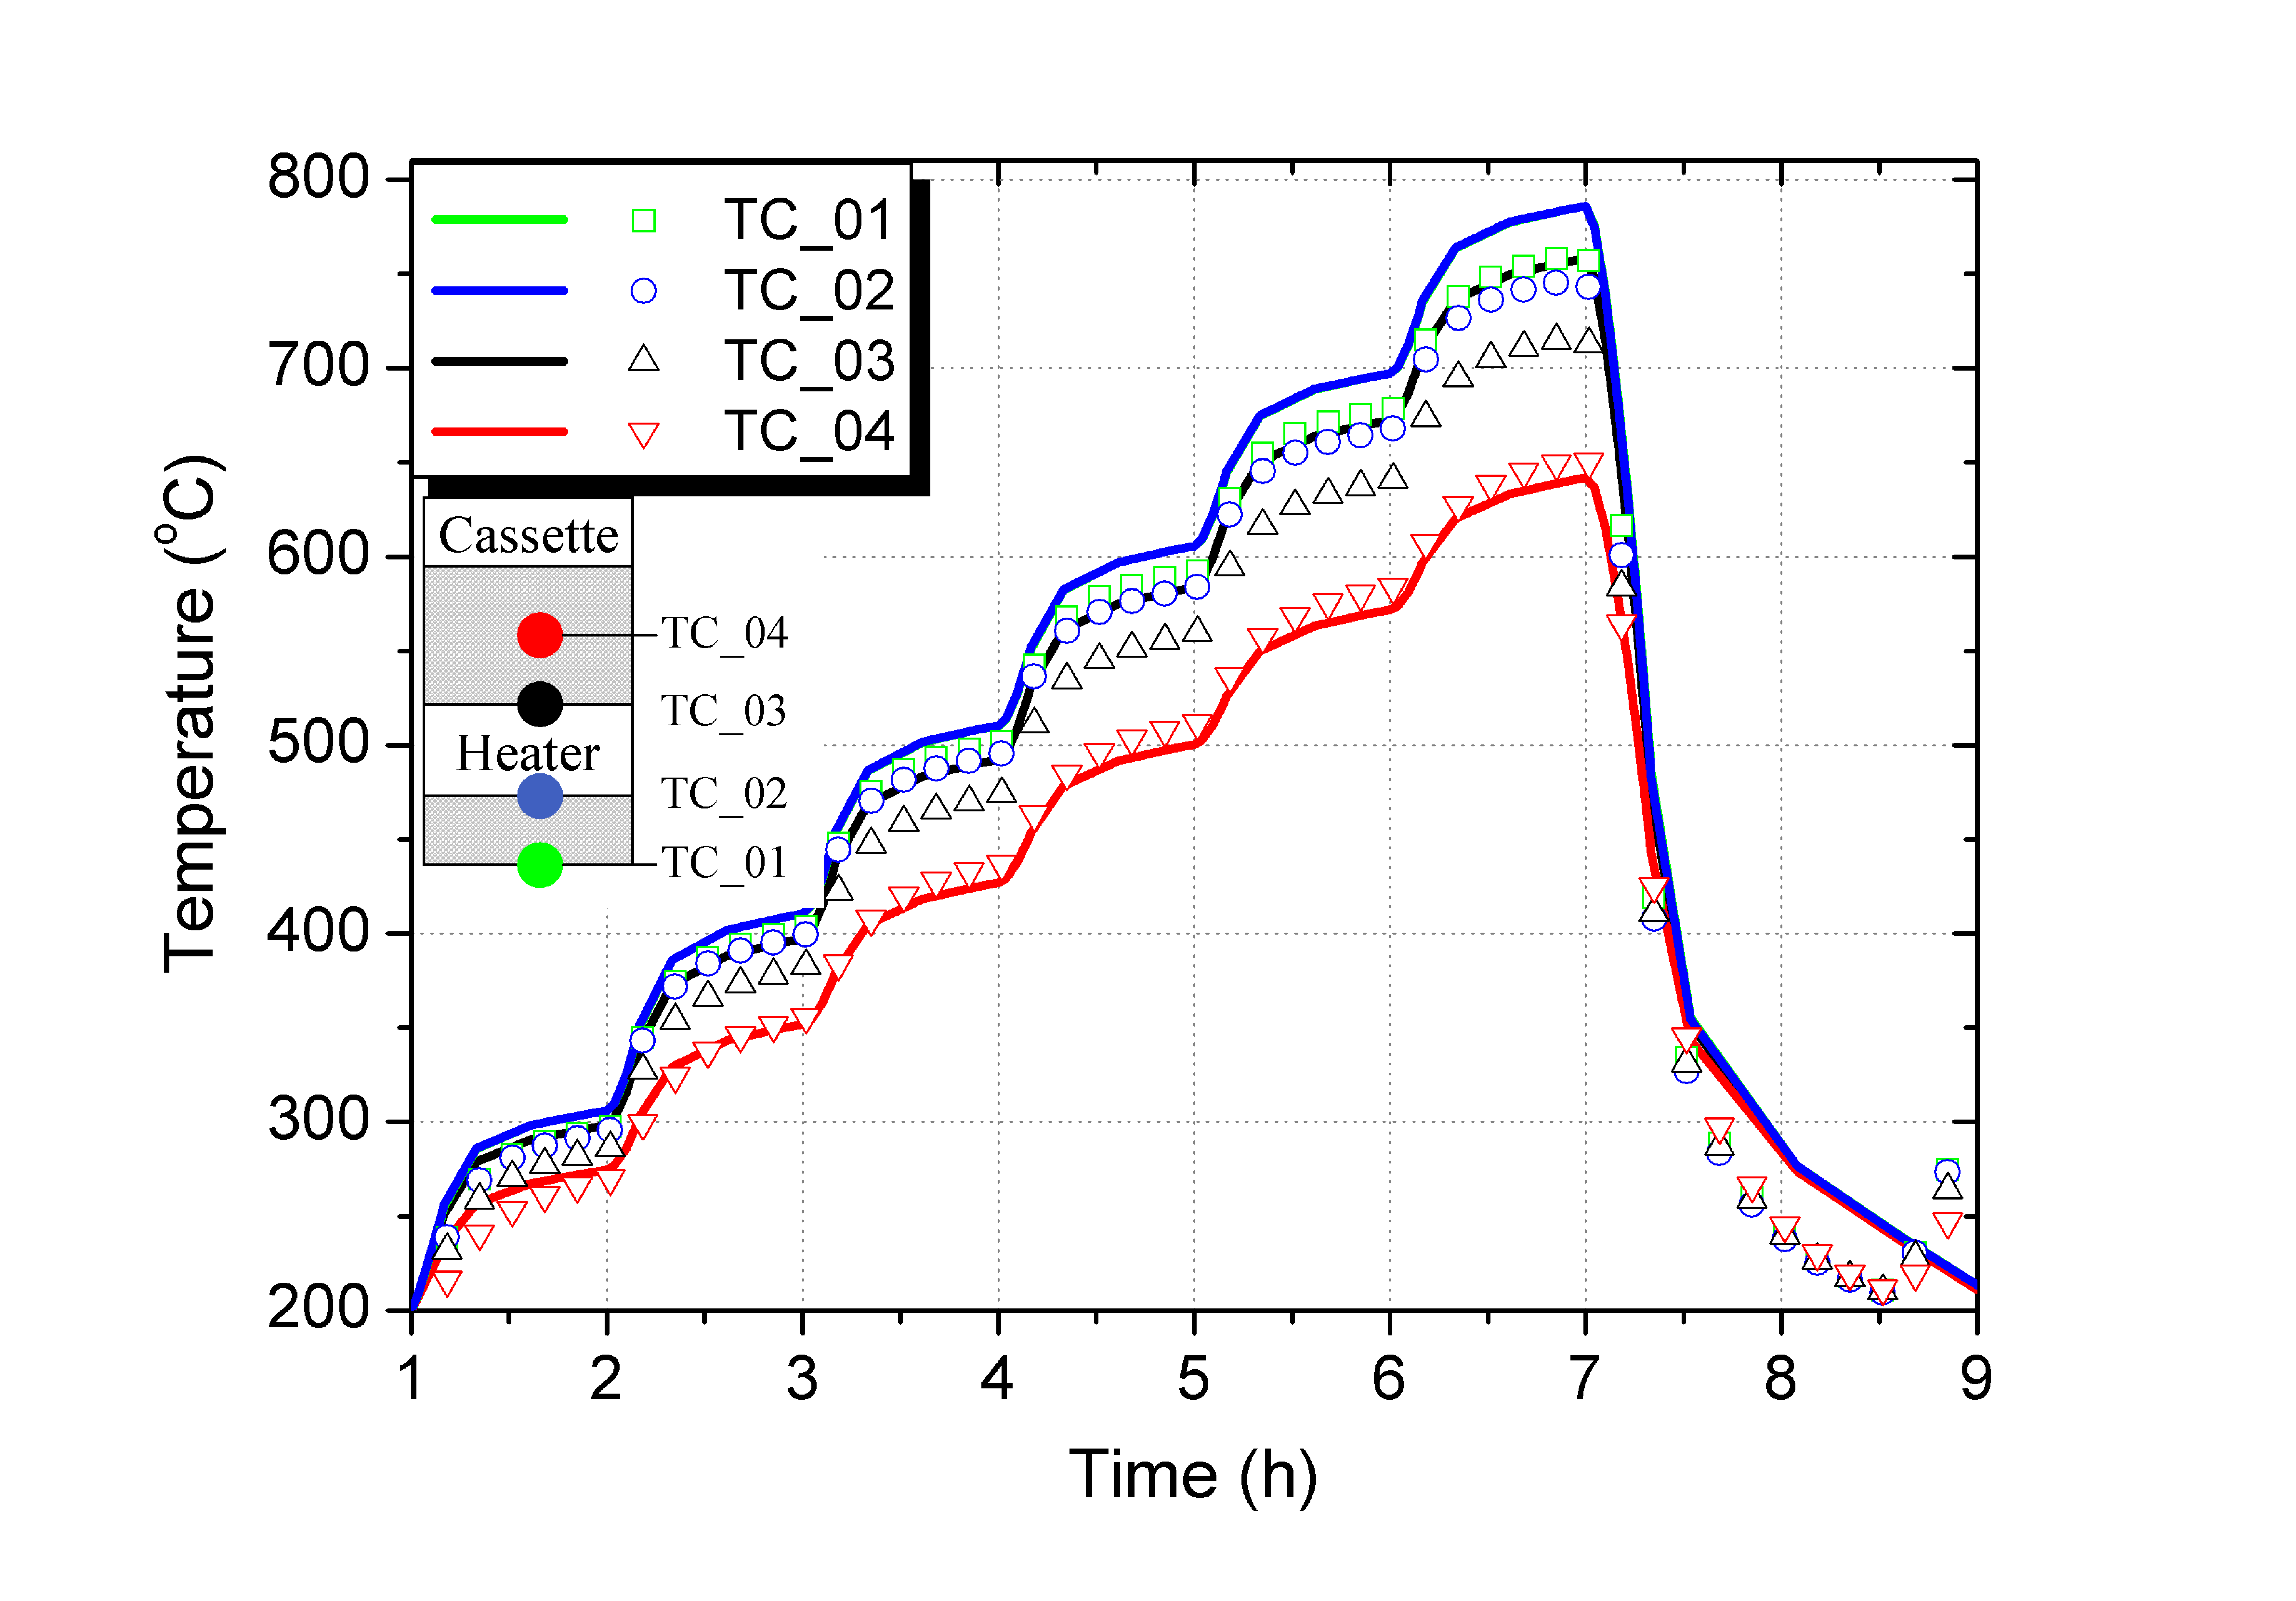
\includegraphics[width=0.5\textwidth]{chapters/figures/Fig-6}
\caption{Results of the FZK benchmarking with HELICA\cite{Gan:2009vn} showing temperature variations with time during a loading cycle (T in $^\circ$C) at 100 mm from FW.}\label{fig:FZK_HELICAa}
\end{figure}

\begin{figure}[t!]
\centering
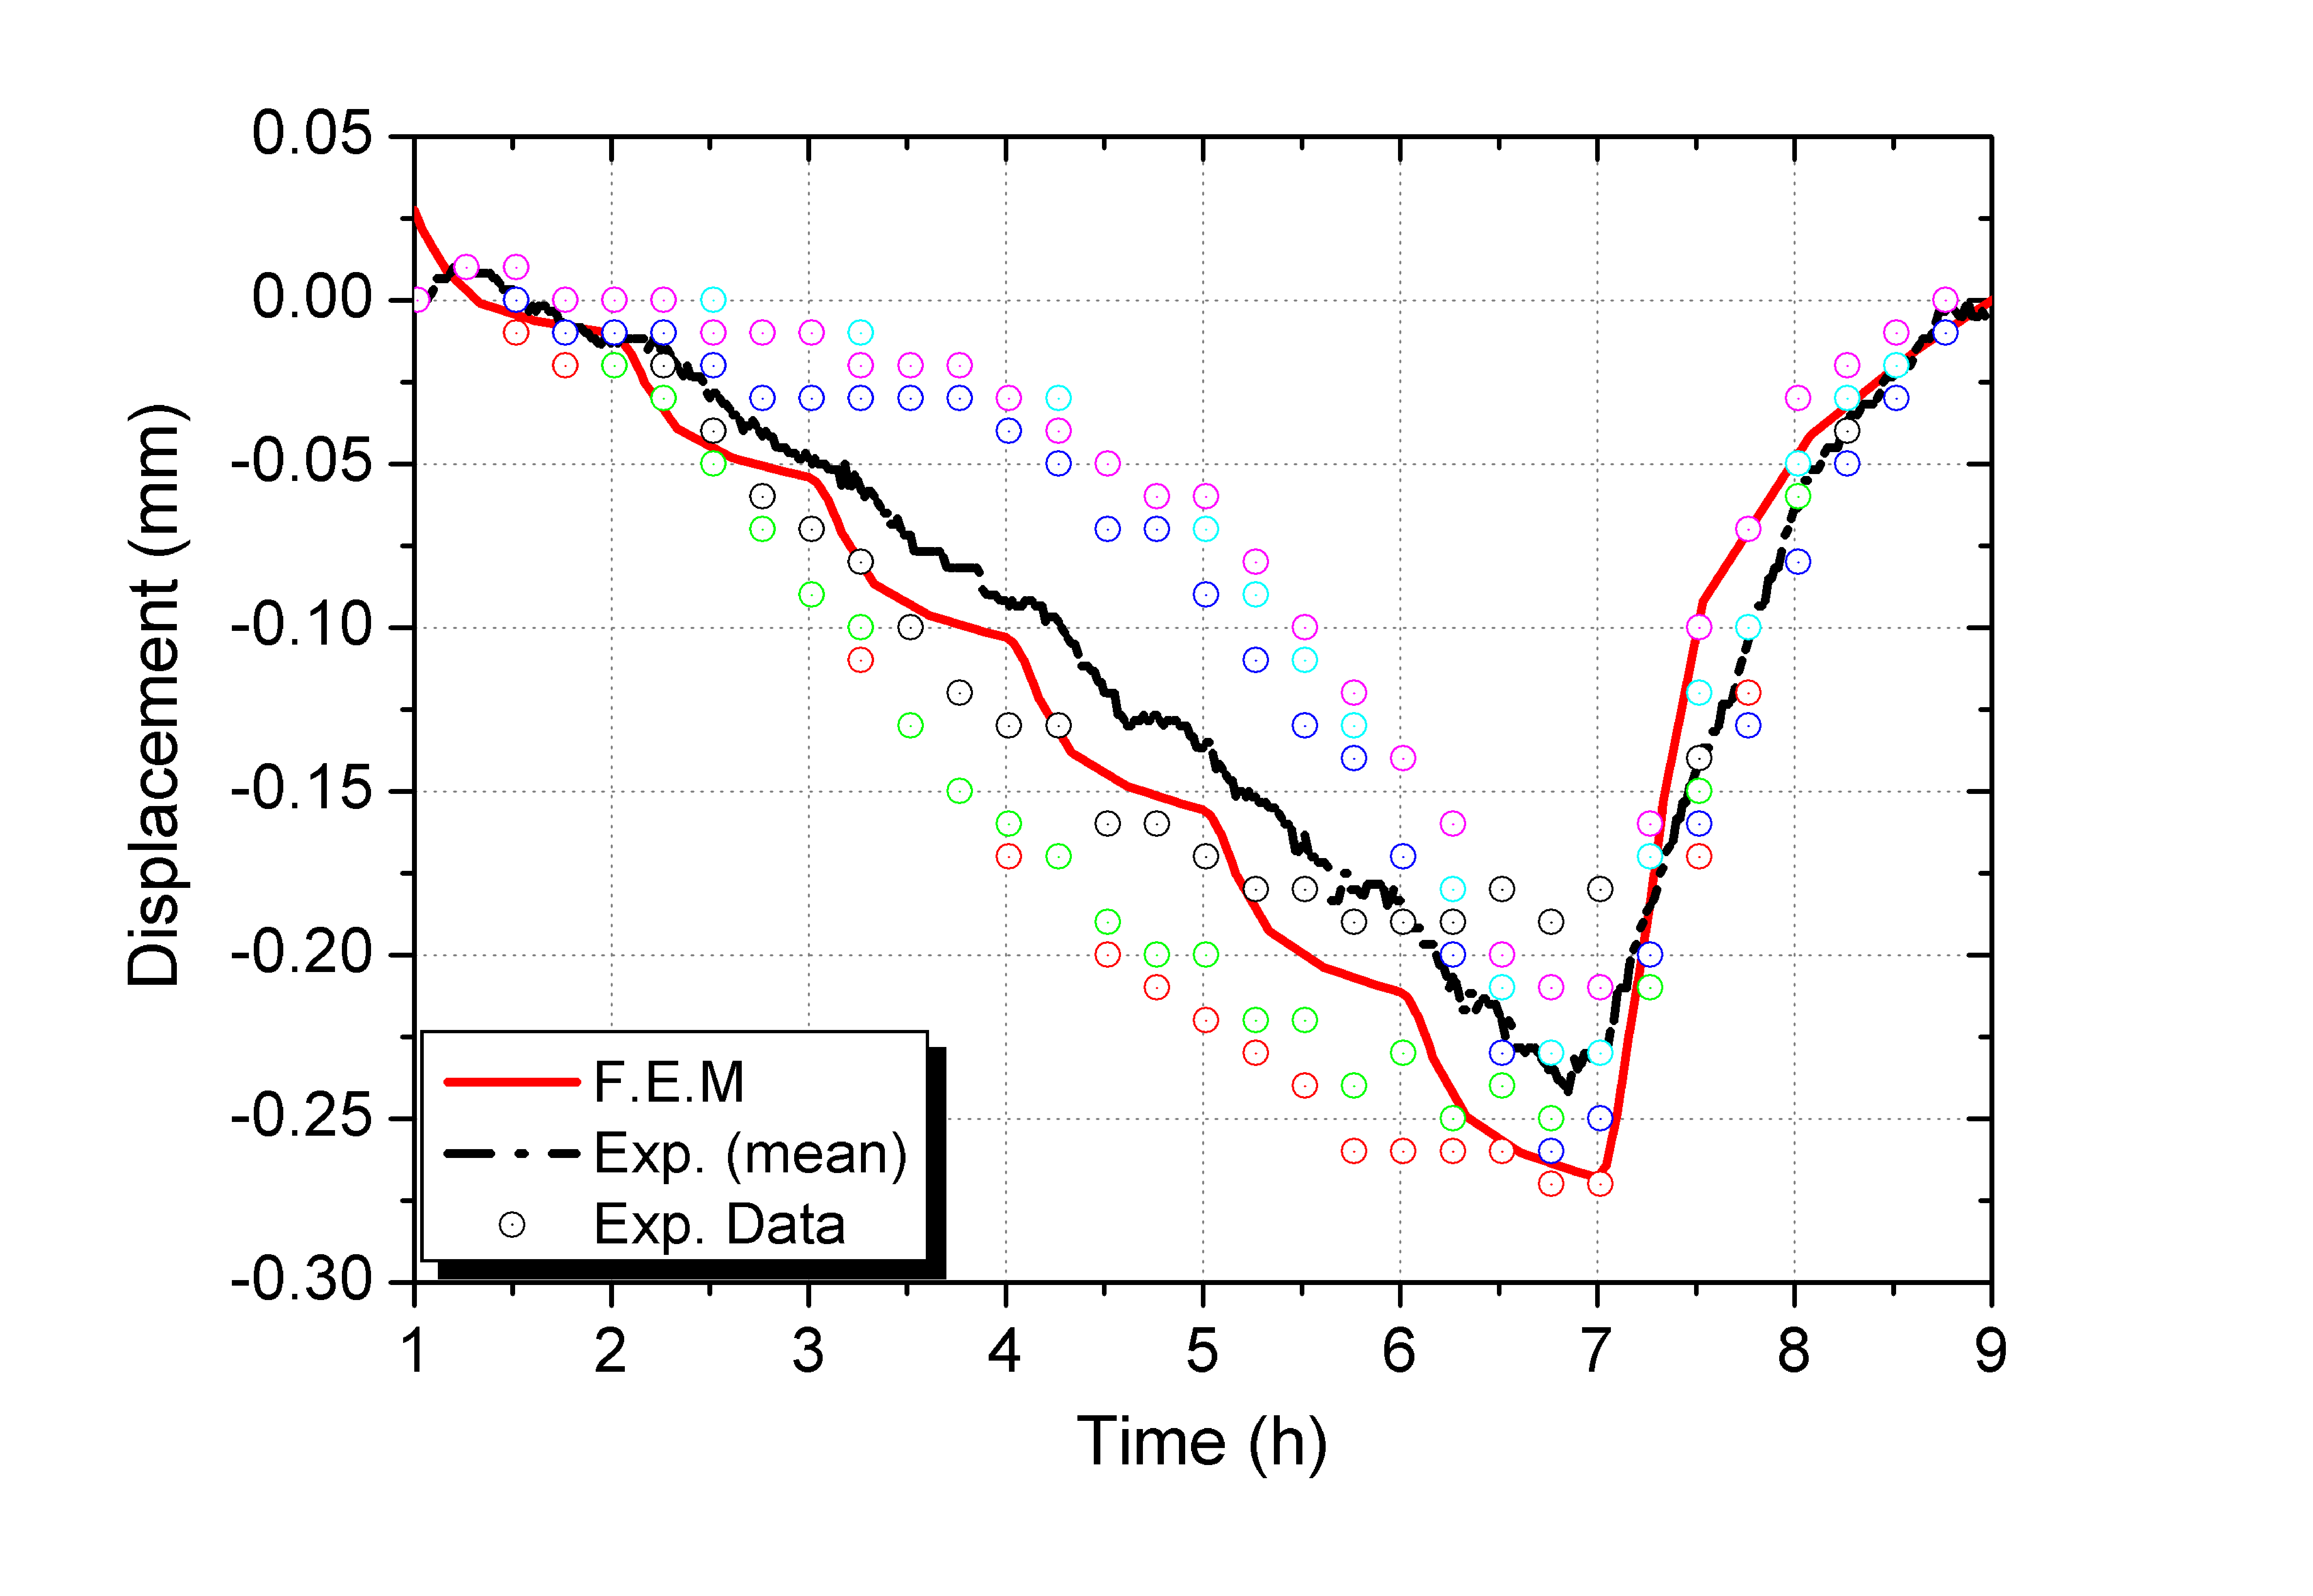
\includegraphics[width=0.5\textwidth]{chapters/figures/Fig-7}
\caption{Results of the FZK benchmarking with HELICA\cite{Gan:2009vn} showing a comparison of displacements (in mm) in HELICA between calculated and measured LVDT values.}
\label{fig:FZK_HELICAb}
\end{figure}

Unfortunately, the ambitions of HEXCALIBER were limited due to the crippling of several heaters. Nevertheless, the limited data was still used in efforts to validate the constitutive relationships of the DIN model. The temperature variations with time were the only major result reported by the ENEA Brasimone team, such as that shown in Fig.~\ref{fig:DIN_HEX}; mechanical results are still forthcoming from the research group. From the comparisons to experimental measurements in HELICA and HEXCALIBER it is encouraging to notice that even in the absence of a creep model, satisfactorily close agreement were seen between computation and measurement. So far, no detailed displacement comparisons have been made to experimental data.

Several important observations are also made from the results of the DIN simulation: (i) three-dimensional effects were important to calculations of the convective energy transport of the helium coolant; future models should continue to be analyzed in three-dimensions; (ii) DIN reports that in HELICA all ceramic beds experience a compressive force everywhere and no gap formation is ever detected. 

In summary, the benchmarking efforts have only recently begun in Europe. A typical pebble bed thermomechanics simulation involves first calculating overall temperature fields of the blanket unit as it undergoes volumetric nuclear heating as well as cooling at the boundaries. The non-linear mechanical analysis is then performed for stress and strain estimations. However, since the effective thermal conductivity of the ceramic breeder pebble bed is, to some degree, dependent on strain, a coupled thermal and mechanical analysis is needed. Additional details on modeling steps can be found in Refs.~\cite{DellOrco:2010zr,DiMaio20081287,DiMaio20101234,Gan:2009vn,Gan:2010lh,dellorco:2006}. The two most developed models, from FZK and DIN, have had their results compared to experimental data and have thus far shown great promise. 

However, it must be noted that the benchmarking efforts are incomplete and inconsistencies between the two models must be explained as they move forward. For example, the model of FZK concluded that a gap appeared between the pebble bed and structural wall, however the model from DIN reported no gap formation. The existence of a gap between pebble bed and structural wall will negatively affect the ability to cool the pebble bed and thereby impact structural and tritium release properties of the bed. That such a discrepancy exists between calculated results of the models on such a critical feature warrants either more benchmarking efforts or a careful deconstruction of the constitutive equations to discover the source of the inconsistency. Future experiments aimed at benchmarking ought to focus on creating apparatus capable of expressing, among other things, when gap formation or pebble failure occurs.


\begin{figure}[t!]
\begin{center}
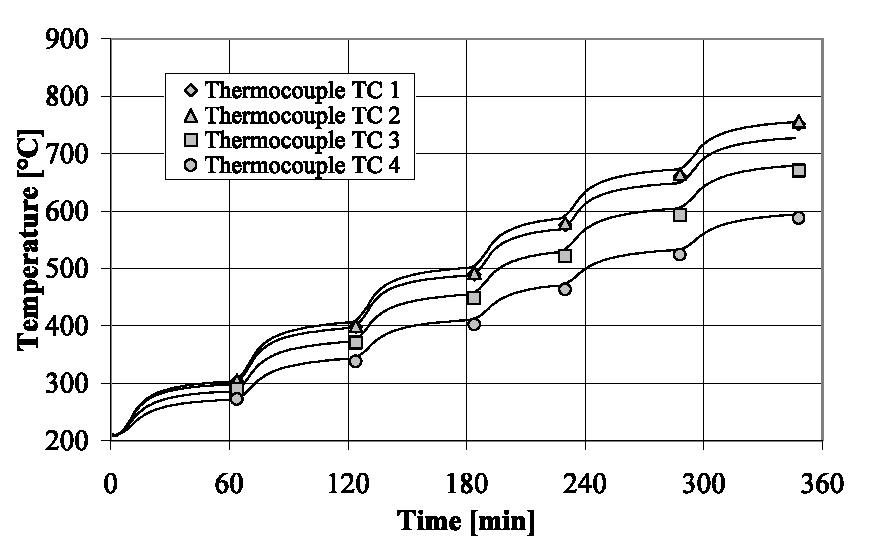
\includegraphics[width=0.4\textwidth]{chapters/figures/Fig-8}
\caption{Exemplary results of the DIN benchmarking with HELICA: Temperature variations with time during a loading cycle at 100 mm from FW\cite{DellOrco:2007hc}.}
\label{fig:DIN_HELICA}
\end{center}
\end{figure}


 \begin{figure}[t!]
\begin{center}
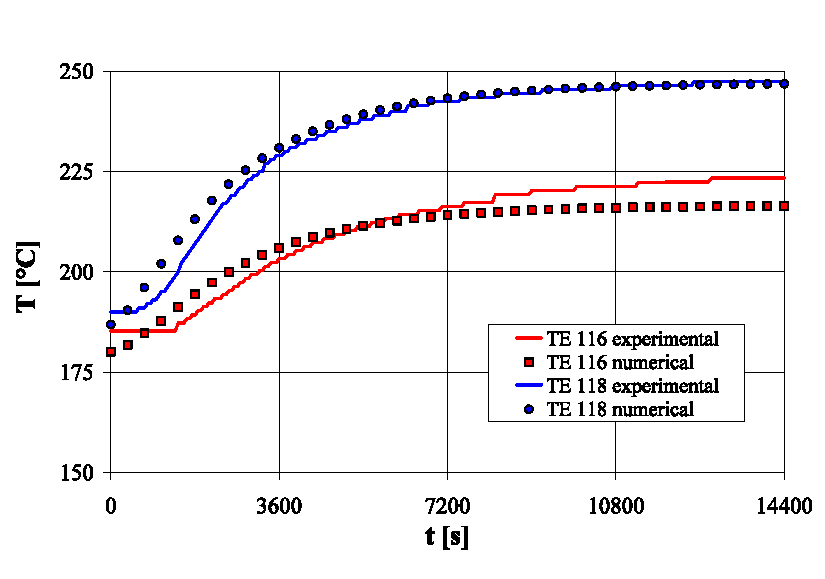
\includegraphics[width=0.4\textwidth]{chapters/figures/Fig-9}
\caption{Exemplary results of the DIN benchmarking with HEXCALIBER : Temperature variations with time during a loading cycle within the first lithium-orthosilicate cell\cite{DellOrco:2010zr}.}
\label{fig:DIN_HEX}
\end{center}
\end{figure}



\subsection{Pebble bed assemblies experiment}
The pebble bed assemblies (PBA) experiment is designed to study the effect of neutron irradiation on the thermo-mechanical behavior of a ceramic breeder pebble-bed under DEMO representative thermo-mechanical loads \cite{Magielsen2007}. This was accomplished via analysis of changes of the in-pile temperature profiles during irradiation as wall as from the post irradiation examination of the pebble bed in the Hot Cells. Within the assemblies, there are four test elements; each resembling a small-scale mock-up of a HCPB TBM with a ceramic breeder pebble bed sandwiched between two beryllium pebble beds. Before irradiation, the beds are pre-compacted with a compressive load of 3 MPa to ensure good settling and contact.  

FEM analysis was performed to study pre-compaction procedures.  During progressive irradiation, temperatures are recorded at several locations in the ceramic breeder bed as well as other critical positions. Reviewing the recorded temperature data, when comparing the temperature in the center of the ceramic breeder pebble bed during later cycles and earlier cycles there appears to be a decrease in temperature for the exact same environmental conditions. Changes in the pebble beds and their characteristics are examined both in-pile by neutron radiography and out-of-pile by e.g. SEM during post-irradiation examination (PIE). The estimated bed height reduction from neutron radiographies over the course of the irradiation has shown 3\% of creep compaction. 

A pebble bed experiencing creep compaction is both becoming more dense as well seeing more-developed inter-pebble conduction paths. The effective thermal conductivity for a creep-compacted ceramic pebble bed is thus expected to be higher than a standard ceramic pebble bed. This phenomenon results in lower temperature gradients and a lower overall temperature magnitude, which is precisely what was observed in the experiment over the course of the cycling. 

During PIE, various microscopy preparation techniques are used to study the deformation state of the pebble beds (signs of creep compaction and sintering), formation of gas gaps between the pebble beds and structural materials, and the interaction layers between eurofer-ceramic and eurofer-beryllium. 

Figure~\ref{fig:pba} shows the cross-section of Li$_2$TiO$_3$ pebbles (left) and Li$_4$SiO$_4$ pebbles (right) post irradiation. Evident in the images is sintering of the lithium titanite and significant fracturing of the lithium orthosilicate pebbles. Importantly, however, it must be noted that the pebble beds performed reliably in spite of the changes displayed in these images cite{magielsen2011}. 


\begin{figure}[t!]
\centering
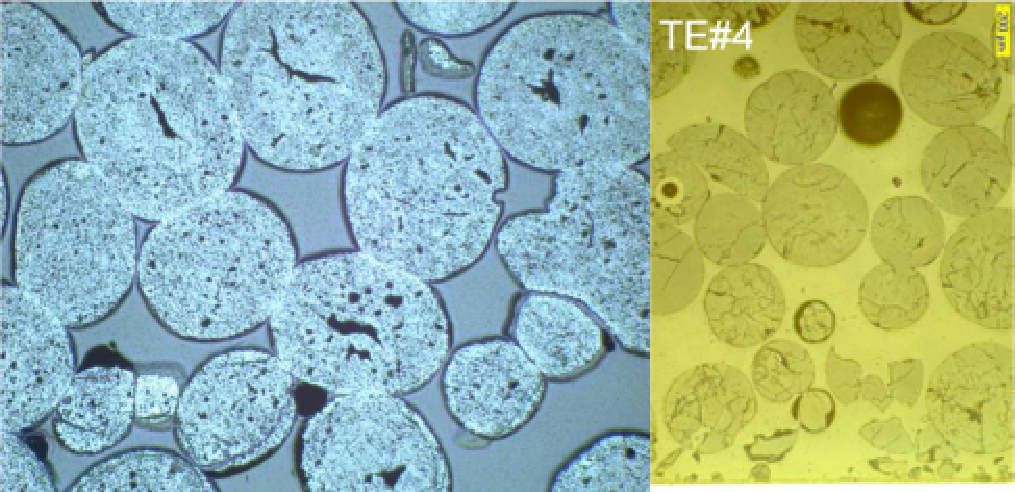
\includegraphics[width=0.5\textwidth]{chapters/figures/Fig-10}
\caption{Notable features of irradiated Li$_2$TiO$_3$ and Li$_4$SiO$_4$ pebble beds from PBAcite{magielsen2011}. (Left) Demonstration of significant sintering of Li$_2$TiO$_3$ pebbles with no fracturing; the visible cracks originated from production and handling. (Right) Demonstration of cracking of Li$_4$SiO$_4$ pebbles.}
\label{fig:pba}
\end{figure}


\subsection{Other thermomechanics characterization experiments}
Coming from the standpoint that strain in a pebble bed is induced by thermal expansion, an experiment was conducted to characterize the pebble bed thermal expansion coefficient \cite{Tanigawa:2007fc}.  The thermal expansion coefficient of a packed \lit pebble bed is measured under a compressive load of 0.1MPa.  The study concludes that for beds with packing factors of 65.3 to 68.5\%, the average thermal expansion coefficient was $(1.4\pm0.2)\times10^{-5}K^{-1}$. This thermal expansion coefficient of the pebble bed was equal to 78\% of that for the bulk material under the conditions used in the study. The reduction in thermal expansion coefficient is less significant than that of the effective modulus, which is more than 2 orders of magnitude smaller than the bulk value. 

The effect of thermal cycling on the packing state is of interest; in particular, it is foreseen that the ITER TBM will be subjected to such conditions. The question that arises is whether a void region will be created under thermal-cyclic loading due to the differential rates of expansion and contraction of the pebble bed and structural containing wall. This uncertainty was first addressed in an experimental set-up involving Li$_2$TiO$_3$ pebbles enclosed by two Kovar flanges while sandwiched between two commercial-grade CVD silicon carbide discs \cite{Calderoni:2006ye}. The set-up allows for generating a high stress through large differential in thermal expansion coefficients. The experimental results indicate that high thermal stresses and deformations are present during the initial thermal cycle of the assembled test article, but are successively alleviated due to a combination of pebble re-arrangement within the bed and creep induced deformation. This suggests that a few thermal cycles under a controlled atmosphere and a compressive load before final assembly of blanket sections would mitigate the severity of the thermal stresses during start-up. This is also shown in a later experiment, in which the increment of compression decreased with each heating cycle and became negligible after 30 cycles \cite{Tanigawa:2010cr}. Extrapolating the finding to a prototypical blanket breeder pebble bed design, the study concludes that for a height of 1 m long pebble bed, a 51 mm high cavity may be generated at the top of the bed with an initial packing of 65\% under thermal cyclic operations.  

\section{Pebble Bed Thermomechanics Summary \& Framework}
The progress already achieved holds the promise of a pebble bed thermomechanics framework that will contribute substantially to the success of the ceramic breeder blanket development. In this framework, the continuum modeling approach using FEM and empirically derived material constitutive equations is capable of correctly characterizing the stress load to which a breeder pebble bed unit may be subject during the operations as shown in Fig.~\ref{fig:framework}. The DEM approach analyzes this load and determines the possibility fraction of pebble cracking based on the crush load data of pebbles or the degree of sintering depending on the local contact stress. The combined analyses warrants a high confidence of success to the assembly and design of breeder units in a blanket.  Experiments should also be conducted to assess the manner of pebble relocations and packing rearrangement when pebble cracking occurs. Since there is no perfect packing state, it is important to learn if the breeder unit will continue to function in accord with the original design goals under all complex operating conditions.  The ultimate objectives of the pebble bed thermomechanics include to delineate a  near-equilibrium packing state as the initial state, quantify breeder unit thermomechanics parameters during operations, understand how these properties vary as packing state alters and the degree of variation, and ensure breeder functions as it is intended to in the fusion operational phase spaces.
\begin{figure}[t!]
\begin{center}
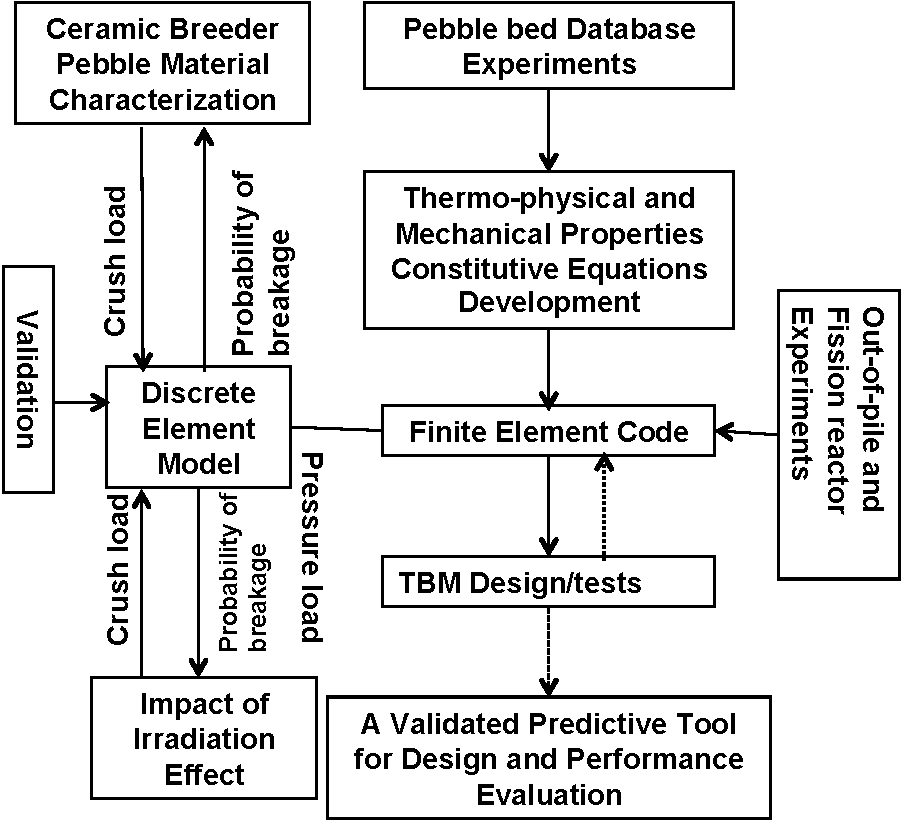
\includegraphics[width=0.5\textwidth]{chapters/figures/Fig-11}
\caption{Example Pebble Bed Thermo-mechanics Research Framework.}
\label{fig:framework}
\end{center}
\end{figure}

This leads to a more reliable blanket design. The analysis has preliminarily defined what peak stress values the breeder unit may be subjected to under the operations (e.g. $< 2-3$ MPa for Li$_4$SiO$_4$ or $< 5$ MPa for Li$_2$TiO$_3$). Since creep will lead to stress relaxation, further development incorporating creep models for high temperature DEM simulation is desired. This may increase the peak stress margin if stress relaxation is taken into account. Despite the scale of the experiments conducted so far, validation experiments are still necessary in regards to current continuum FEM models. Moreover, validation and refinement of simulations with regards to pebble damage crush properties are desired in particular in view of damage mechanisms.  There may be merits to perform crush load tests for irradiated pebbles at operating temperature ranges (room to 850/900 $^\circ$C). It holds forth promising on the continued pebble bed thermomechanics study in fine details a higher confidence to the ceramic breeder lifetime performance in a blanket.  The quest is to define and search a persistent ceramic breeder packing state throughout the blanket lifetime. 
